% POT.tex      pdflatex ZhCvGo15
% Diffuse globally, compute locally: a cyclist tale
% Tingnan Zhang, Daniel I. Goldman and Predrag Cvitanovi\'c

% \subsection{Periodic orbit theory}
% \label{s-POT}

\Po\ theory of deterministic diffusion, introduced in
\refrefs{art91,LorentzDiff}, exploits the fact that the periodic Lorentz
gas can be constructed by putting together translated copies of an
elementary cell. Therefore quantities characterizing global dynamics,
such as the Lyapunov exponents and the diffusion tensor, can be computed
from the dynamics restricted to the elementary cell, as shown numerically
in \refref{CGS92}.

In \refrefs{art91,LorentzDiff,CGS92,Artuso94,CBdiffusion} it was shown that
deterministic diffusion tensor in the {\em periodic} Lorentz gas can be
expressed in terms of (relative) \po s, and exact \cycForm\ for such
global dynamical averages as Lyapunov exponent and diffusion tensor were
derived, using only the dynamics in the \emph{elementary cell}, which we discuss now. For any
dynamical system that has translational symmetry, the full state space
$\hM$ (i.e., both spatial coordinates and momenta) has aperiodic tiling
\[ %beq
\hM=\bigcup_{ \hn \in T} \pS_{\hn},
\] %eeq
by {\em translating} $\pS_{\hn}$ of an {\em elementary cell} $\pS$, with
$T$ the abelian group of lattice translations.

\begin{figure}[htbp]
	\begin{center}
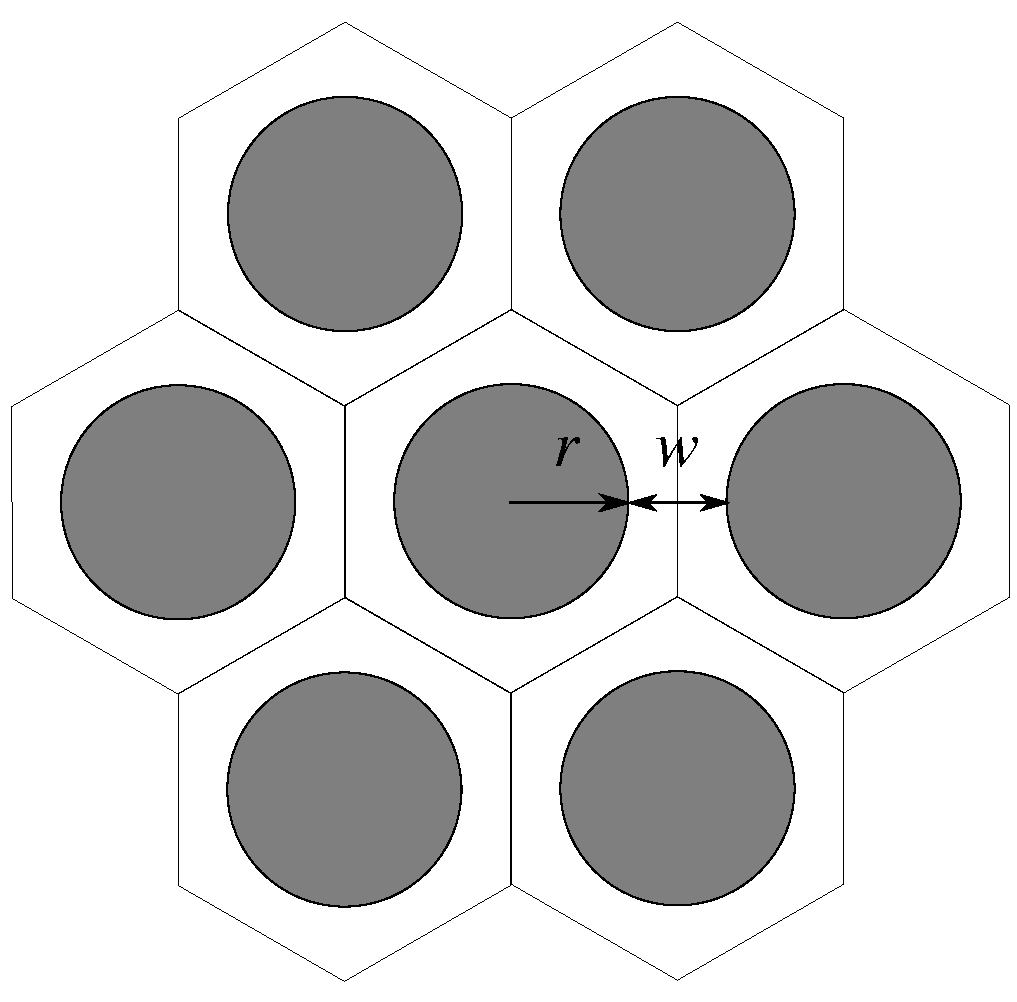
\includegraphics[width=0.25\textwidth]{diffuseLorentzGasParams}
	\end{center}
	\caption[]{\label{fig-LorentzGasParams}
		An elementary cell and its six unit translations. The ratio of
		distance $w$ between the nearest pair of disks to the    disk radius
		$r$ determines the dynamical properties in the system.
	}
	\TZ{2016-01-15}{This figure is also generated by me.}
\end{figure}

In the context of triangular Lorentz gas system, the elementary cell is the hexagon centered at the scatterer, see \reffig{fig-LorentzGasParams}. The
dynamics restricted inside the elementary cell is understood as the periodic
boundary condition: when the particle leaves the edge of the hexagon cell, it
immediately enters the region again from the opposite edge. The transition between finite and and infinite horizon is controlled by the ratio of $w/r$, where $w$ is the gap between nearest pair of disk and $r$ the radius of the disk. The horizon is finite for $w/r < 4/\sqrt{3}-2 = 0.3094\dots$.

    \PC{2013-02-03}
    { Roberto says we must
incorporate kneading determinants from
Cristadoro\rf{ArtCri03,Cristad06,CriKnDeEsp12}.
    }

%    \PC{2015-10-21}
%    {edits based Cvitanovi\'c,  Eckmann,and Gaspard\rf{LorentzDiff}}
%In \refrefs{art91,LorentzDiff,CGS92,Artuso94,CBdiffusion}  an explicit
%connection between the global diffusion and the dynamics restricted to
%an elementary cell.
%Our method applies to any  hyperbolic dynamical system that is
%a periodic tiling $\hM=\bigcup_{ \hn \in T} M_{
%\hn}$
%of the dynamical phase space $\hM$ by {\sl translates}
%$M_{\hn}$
%of an {\sl elementary cell} $M$, with $T$ the abelian group of lattice
%translations.
%Furthermore, each elementary cell may be built from a
%{\sl fundamental domain}
%$\tM$
%by the action of a discrete (not necessarily Abelian) group $G$.


Machta and Zwanzig\rf{MacZwa83} have given numerical results
for the diffusion constant in Lorentz gases,  as well as
estimates based on a random walk approximation. We shall follow
their notation and fix the radius of the disks to 1,
assume unit particle speed.

We now relate the dynamics in $\pS$ to diffusive properties of the
Lorentz gas in $\hM$. Let $\hx(t)\,=\,\hflow{t}{\hx_0}$ denotes the point
in the global space $\hM$ reached by the flow in time $t$.
$x(t)\,=\,\flow{t}{\xInit}$ denotes the corresponding flow in the
elementary cell; the two are related by
\beq
\hn_t(\xInit)=\hflow{t}{\xInit} - \flow{t}{\xInit} \in T \,,
\ee{l-diff-hatn1}
the translation of the endpoint of the global path into the elementary cell $\pS$.

Fix a vector $\beta \in \reals^d$, where $d$ is the dimension of
the{\statesp}. We will compute the diffusive properties of the Lorentz
gas from the leading eigenvalue of the Rulle-Frobenius-Perron \evOper\
\beq
\eigenvL(\beta)\,=\, \lim_{t \rightarrow \infty} \frac{1}{t} \log \langle
e^{\beta \cdot (\hx(t) -x) } \rangle_\pS ~, \quad
\label{eq-diff-1}
\eeq
where the average is over all initial points in the elementary cell, $x
\in\pS$. If all odd derivatives vanish by symmetry, there is no drift and
the second derivatives

\bea
2d D_{ij} &=& \left . {\frac{\partial}{\partial \beta_i}} {\frac{\partial}
{\partial \beta_j}} \eigenvL(\beta)\right\vert_{\beta=0}\\\nonumber
&=&\lim_{t\rightarrow
\infty} {\frac{1}{t}} \langle {(\hx(t) -x)_i (\hx(t) -x)_j } \rangle_\pS \,,
\eea

yield a diffusion matrix.  This symmetric matrix can, in general, be
anisotropic (\ie, have $d$ distinct eigenvalues and eigen\-vectors). The
spatial diffusion constant is then given by the Einstein relation
\beq
D\,=\,{1\over 2 d} \sum_i \left .{{\partial}^2 \over {\partial
      \beta^2_i}} \eigenvL(\beta)\right |_{\beta=0} \,=\,
\lim_{t\rightarrow \infty} {1\over{2d t}} \langle {(\hat{q}(t) -q)^2 }
\rangle_\pS~ ~,
\eeq
where the $i$ sum is restricted to the spatial components $q_i$ of
the {\statesp} vectors $x=(q,p)$, \ie, if the dynamics is Hamiltonian, the
sum is over the $d$ degrees of freedom.
\PC{2014-11-18}{reinstate mass, velocity, size to get $\beta$, $m$, $\sigma$
    dependencies right?}

\TZ{2016-01-15}{Now we should introduce the poincare return map because will work on both the map and the continuous flow. Explain why use poincare return map and what kind of section do we choose.}

It was shown in \refref{CGS92} that the ensemble average in~\refeq{eq-diff-1} can be written as an integral over the elementary cell
\beq
\langle e^{\beta\cdot(\hx(t)-x)} \rangle
   = \frac{1}{\vert \pS \vert}\int_{x,y\in \pS} dxdy {\cal L}^t(y,x),
\eeq
given the linear \evOper
\beq
{\cal L}^t(y,x) = e^{\beta\cdot(\hx(t)-x)}\delta(y-x(t))\,,
\label{eq-eOper}
\eeq
for the flows and
\beq
{\cal L}^n(y,x) = e^{\beta\cdot(\hat{f}^n(x)-x)}\delta(y-f^n(x))\,,
\label{eq-eOperDisc}
\eeq 
for the poincare return maps.

For sake of simplicity, we will proceed with the derivation for the discrete maps and eventually generalize to the continuous version.

\TZ{2016-01-15}{Now we connect the linear operator with the spectrum, and evaluate the trace, for the poincare return maps.}


Generalization to continuous time\rf{bowen,pexp} amounts to the replacement
%$ z\,=\,e^{-s} $,
$ z^{\period{p}} \rightarrow e^{-s \period{p}} $,
where $\period{p}$ is now the (not necessarily integer)
%{\sl time-}
period of the prime cycle $p$:
$$
Z(\beta,s)\,=\,\prod_{p\in\PP} \exp \left( - {
 \sum_{r=1}^\infty {1 \over r}
 { e^{(\beta \cdot \hn_p- s \period{p}) r } % z^{n_p r}
 \over { | \det \left( {\bf 1}-{\bf J}_p^{r} \right) | } }
 } \right)
\,\, .
%Eq.~(14)
$$


% As we are concerned with the long time behavior,
% this problem can be circumvented
% by replacing $ \hf^t(\tx{\tpk}) $ by the mean
% drift in the $t \rightarrow \infty$ limit.
% $ \hf^t(\tx{\tpk}) $ is a translation in $\hM$ for each
% complete cycle $p$ in $M$, so we replace
% \bea
% \hf^t(\tx{\tpk}) - \tx{\tpk}
% \,\Longrightarrow \,
% &&
% { { \hf^{m_p t}(\tx{\tpk}) - \tx{\tpk} }
% % \over         m_p
% }
%    % \,\equiv \, r {\tilde n}_{\tp} (\tx{\tpk})
% \continue
%t &=& r \period{\tilde{p}}, \quad m_p = \period{p}/\period{\tilde{p}} \quad \tx \in \tp \,\, ,
% \eea
% in Eq.~(240).
% The magnitude of ${\tilde n}_{\tp}(\tx{\tpk})$, the mean
% global drift per one traversal of the fundamental cycle $\tp$, is
% independent of the starting point, but its direction is not; the
% reason is that each fundamental domain cycle corresponds to a set of
% trajectories in $\hM$.
% The ${1 \over {|G|}} \sum$ average in
% Eq.~(240) then generates all distinct global drift
% directions, so we can again replace the
% sum over cycle points by the factor $\period{\tilde{p}}$, and obtain the
% $Z$ function Eq.~(14) for the $\alpha $ irreducible subspace
% $$
% Z(\beta,s)_\alpha\,=\,\prod_{\tp \in \t{\cal{P}} } \exp
% % \left( -
%  % \sum_{r=1}^\infty {1 \over r}
% % {{
%  % \chi_\alpha(h^r_{\tp})
%  % }
% % \over
% % { | \det \left( \bf{1}-\t{\bf J}_{\tp}^{r} \right) | }
% % }
% % e^{ ( \beta \cdot {\tilde n}_{\tp} - s \period{\tilde{p}}) r}
%  % \right)
% \,\, .
% Eq.~(24)
% $$
% $\hn_{\period{\tilde{p}}}(\tx_k)$
%%{\tt NOnsense...}
% The leading eigenvalue of the
%unsymmetrized
% operator Eq.~(8) is
% the leading eigenvalue of the symmetric subspace for which
% $\chi_\alpha(g)=1$ for all $g \in G$.
%
%The interesting dynamical averages is determined by the spectrum of the operator
%\beq \det(\eigenvL - \Lop) \,=\,\prod_{p} \exp \left(
%  - { \sum_{r=1}^\infty {1 \over r} { e^{(\beta \cdot \hn_p- s
%        \period{p}) r} \over \oneMinJ{r} }
%  } \right) \,,
%\ee{lor-diff-14}
%or the corresponding \dzeta\
\beq
1/\zeta(\beta, s)\,=\,\prod_{p}\left( 1 - \frac{e^{(\beta \cdot \hn_p-
      s \period{p})}}{|\ExpaEig_p|} \right) ~,
\label{zeta-diff}
\eeq
where $\period{p}$ is the period of the cycle and $\ExpaEig_p$ the
product of expanding eigenvalues of the cycle\rf{DasBuch}.

The \dzeta\ \cycForm\ for the diffusion constant, zero mean drift
$ \expct{ \hat{x}_i } = 0 \,, $ is given by
 \beq D \,=\,{1 \over 2 d}
{ \expct{\hat{x}^2}_\zeta \over \expct{\period{}}_\zeta } \,=\,{1
  \over 2 d } \, {1 \over \expct{\period{}}_\zeta} \sumprime
\frac{(-1)^{k+1} (\hn_{p_1}+ \cdots+ \hn_{p_k})^2}
{|\ExpaEig_{p_1}\cdots \ExpaEig_{p_k}|} \, ,
\label{eq-ecDiffCoef}
\eeq
where the sum is over all distinct non-repeating combination of prime
cycles (in the elementary cell). The derivation is standard, still the
formula is strange.Diffusion is unbounded motion across an infinite
lattice; nevertheless, the reduction to the elementary cell enables us to
compute relevant quantities in the usual way, in terms of periodic
orbits.
